
In this chapter, we aim to characterise transcript degradation and read truncation from long-read RNA-seq data. Transcript degradation from the 5' end results in truncated reads and a decrease in coverage with increasing distance from the 3' end for a given isoform. Thus, even though the observed degradation occurs from the 5' end, it is helpful to characterise degradation as the resultant decrease in coverage from the 3' end. We formalize the notion of degradation by defining the \textit{degradation rate}. 
\begin{definition}[Normalized coverage]
Let the maximum coverage over an isoform be $\mathrm{cov}_{\mathrm{max}}$ and the coverage at base $b$ be $\mathrm{cov}_b$. The normalized coverage of the isoform at base $b$ is defined as 
\begin{equation}
    \mathrm{ncov}_b=\frac{\mathrm{cov}_b}{\mathrm{cov}_{\mathrm{max}}}
\end{equation}
\end{definition}
\begin{definition}[Degradation rate]
Let $\mathrm{ncov}$ be the normalized coverage over an isoform, and $x$ be the distance in kb from the 3' end. The degradation rate of an isoform is defined as the rate of change in normalized coverage with respect to distance in kb from the 3' end of the isoform:
\begin{equation}
    d=\lim_{\Delta x\rightarrow 0} \frac{\Delta \mathrm{ncov}}{\Delta x}
\end{equation}
The degradation rate of an isoform at a base $b$ with distance $x_b$ away from the 3' end is the value of this limit evaluated at $x=x_b$. 
\end{definition}
Intuitively, the degradation rate can be interpreted as the gradient of the plot of normalized coverage against distance from the 3' end. We will refer to this plot as the \textbf{degradation curve}. To illustrate this, we visualise degradation curves for a hypothetical isoform of length 2 kb with different degradation rates (Fig. \ref{fig:sec-2-hypo}).  
\begin{figure}[H]
    \centering
    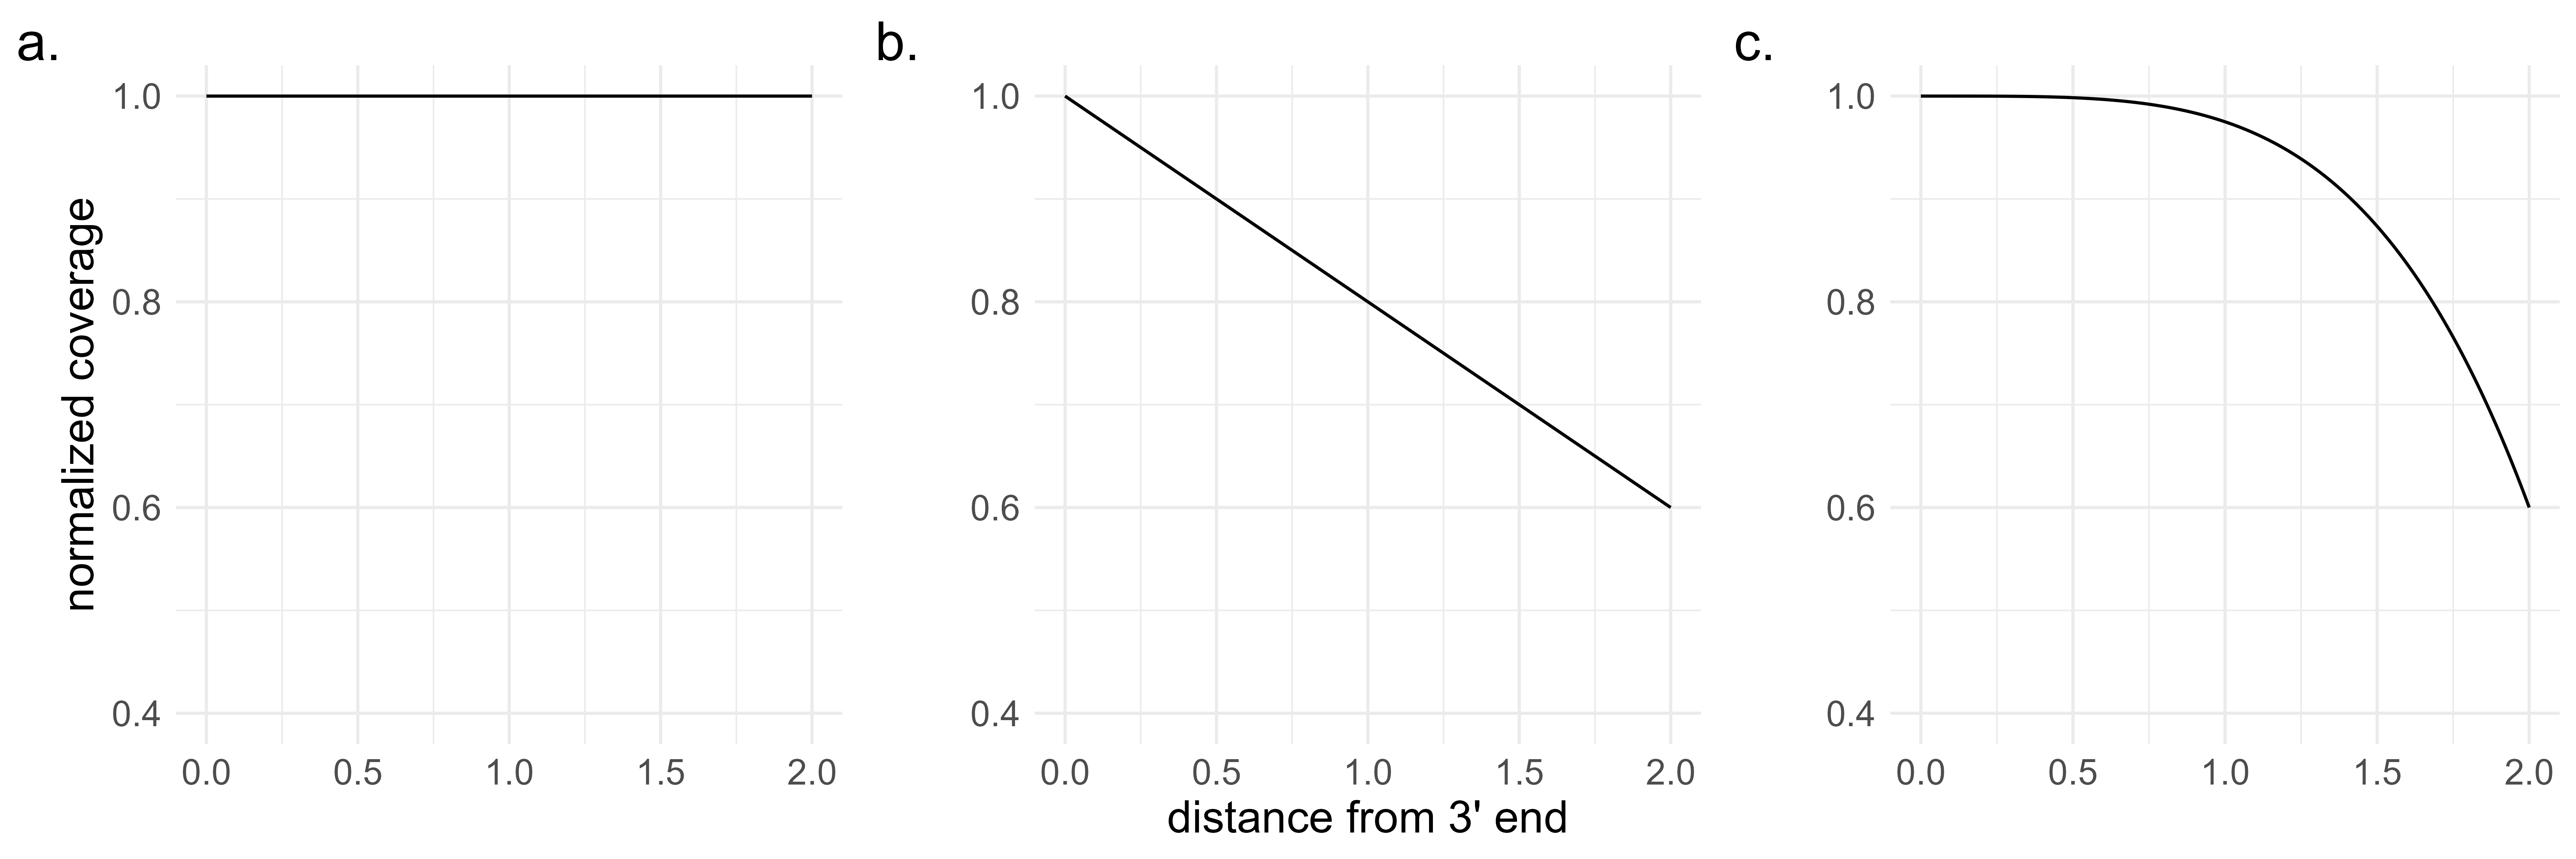
\includegraphics[width=\textwidth]{figures/sec-2-hypo.png}
    \caption[Normalized coverage plots for a hypothetical isoform]{Normalized coverage plots for a hypothetical isoform of length 2 kb illustrating different degradation rates. \textbf{a.} Degradation rate is 0. \textbf{b.} Degradation rate is constant (0.2). \textbf{c.} Degradation rate is variable.}
    \label{fig:sec-2-hypo}
\end{figure}
In Fig. \ref{fig:sec-2-hypo}a, the degradation rate or gradient is 0, implying that all reads from the isoform are full-length, with no drop in coverage over the isoform body. Conversely, in Fig. \ref{fig:sec-2-hypo}b, the gradient is a constant value of 0.2 over the isoform body, implying that for every 1 kb from the 3' end, normalized coverage drops by 0.2. The last plot in Fig. \ref{fig:sec-2-hypo}c shows variable gradient over the isoform body. In particular, the gradient is low in magnitude towards the 3' end and increases with distance from the 3' end.  

In the following sections, we first describe a coverage-based approach for characterising degradation in long-read direct RNA-seq data, and validate this approach with simulated data where the degradation is known. We then examine degradation in real data, characterising degradation by isoform features and in sequencing spike-ins. Finally, we develop a method for efficient read length-based degradation estimation that can be used for obtaining degradation-aware isoform abundance estimates.

\section{Coverage-based degradation estimation}\label{sec:deg-est}

We first sought to determine if patterns of degradation were consistent across transcript isoforms for a given direct RNA-seq dataset. To that end, we selected single-isoform, multi-exon genes from GRCh38 reference annotations, and further restricted the set of isoforms to those that do not intersect with any other annotated features in reference annotations. We refer to these as \textbf{lone isoforms}. Estimating bias from lone isoforms reduces ambiguity in the isoform of origin of the reads we use to estimate bias; such approaches were also adopted in \cite{Roberts2011} and \cite{Love2016} for bias estimation in short-read data. Filtering yielded approximately 5,000 lone isoforms. For each of these isoforms, we obtained coverage over the isoform body using the \texttt{genomecov} module from bedtools (v.2.27.1). Next, we further apply a median coverage filter, filtering out lone isoforms with low median coverage (min median coverage = 10). Finally, a degradation curve is fitted to the data with a smoothing spline.  

To validate this approach, we simulated two datasets where the expected degradation rates for all isoforms is constant ($\mathbb{E}[d]\in\{0.2,0.4\}$, see Appendix \ref{ap:sim-deg-reads} for more details on degraded read simulation). Visualising the degradation curves for each isoform, we observed noise in the form of deviation from the expected degradation curve, likely due to sampling noise in the simulation data generation process. This noise can be mitigated by computing a global degradation curve across all isoforms (red line, Fig. \ref{fig:cov-sim}). We find that the global degradation curves reflect the known degradation rates from the simulated data qualitatively (Fig. \ref{fig:cov-sim}). In addition, we assessed the global degradation curves quantitatively by computing the average gradients of each curve, and found good agreement between the estimates and the expected degradation ($\mathbb{E}[d]$ = 0.2, estimated = 0.201; $\mathbb{E}[d]$ = 0.4, estimated = 0.403).

We applied this approach in real direct RNA-seq data from the SG-NEx project. Within each sample, we found consistent patterns of degradation across isoforms (Fig. \ref{fig:cov-real}). However, we note that for most real datasets, filtering for lone transcripts and by median coverage yields very few isoforms remaining for estimating degradation rates. For instance, in a HepG2 sample (Fig. \ref{fig:cov-real}a), we obtained only 57 isoforms, while in a MCF7 sample (Fig. \ref{fig:cov-real}b), we obtained only 52 isoforms. 

\begin{figure}[H]
    \centering
    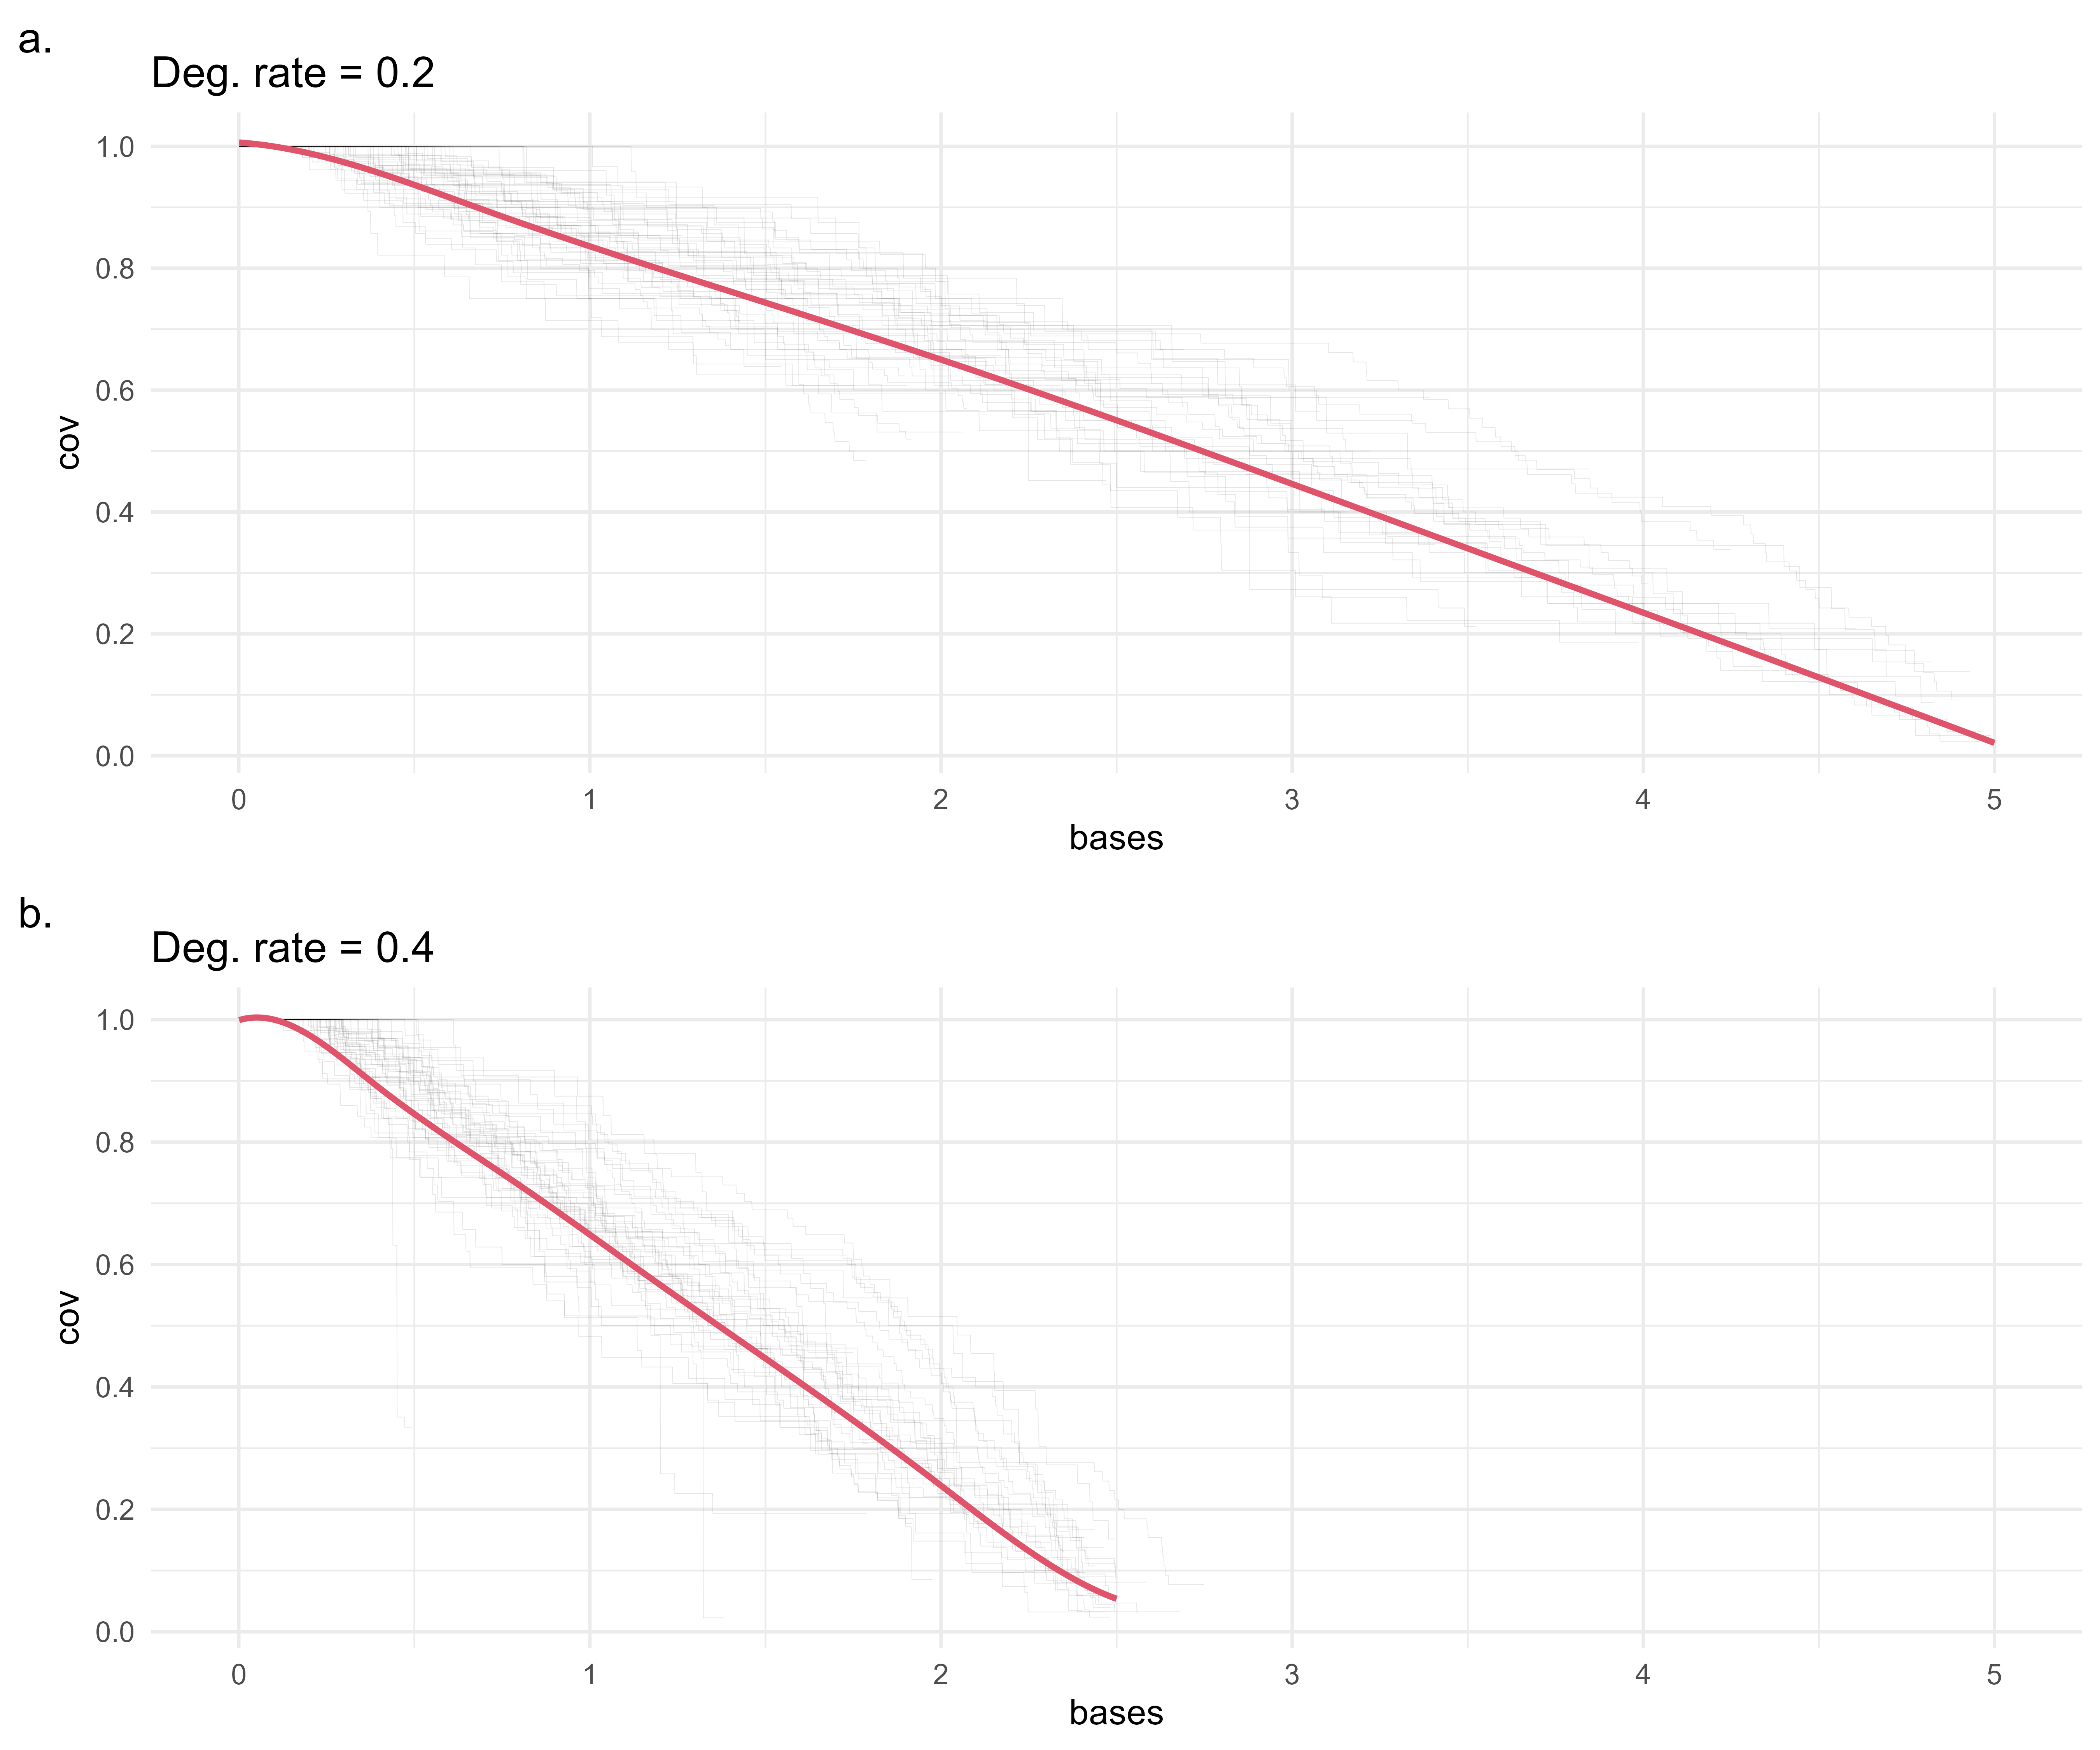
\includegraphics[width=\textwidth]{figures/sec-2-cov-sim.png}
    \caption[Degradation curves on simulation datasets based on coverage]{Degradation curves on simulation datasets based on coverage. \textbf{a.} Degradation curve for dataset with $\mathbb{E}[d]$ = 0.2. Coverage drops close to 0 at 5kb with a degradation rate of 0.2. \textbf{a.} Degradation curve for dataset with $\mathbb{E}[d]$ = 0.4. Coverage drops close to 0 at 2.5 kb.}
    \label{fig:cov-sim}
\end{figure}

\begin{figure}[H]
    \centering
    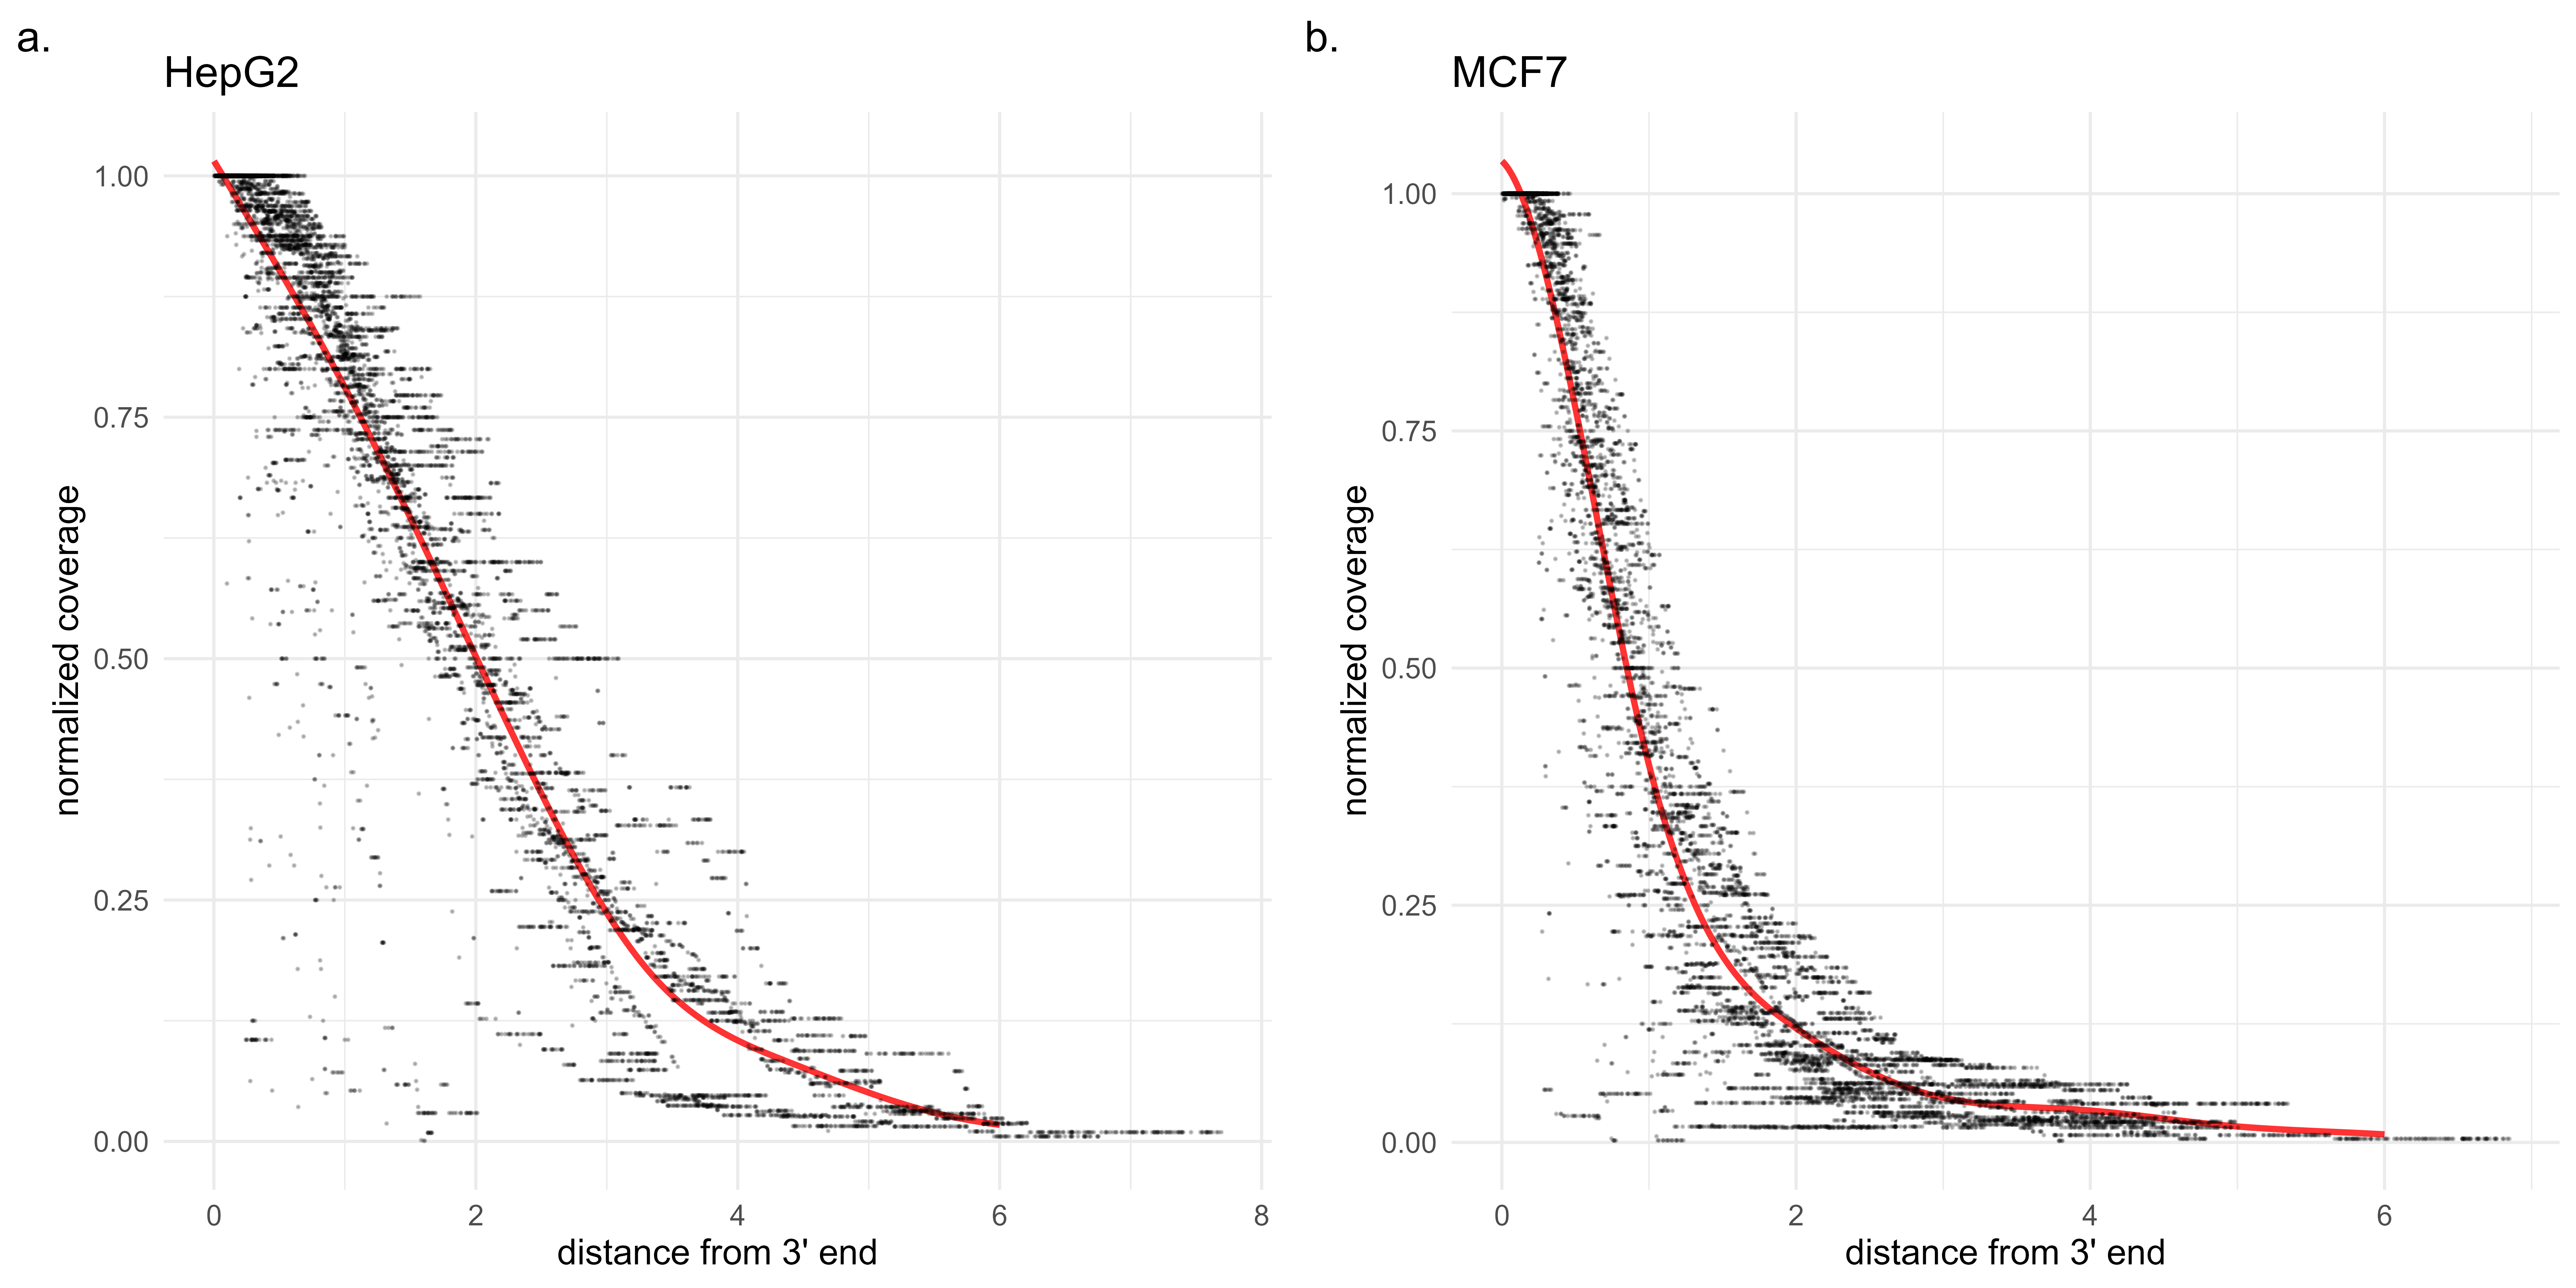
\includegraphics[width=\textwidth]{figures/sec-2-cov-real.png}
    \caption[Degradation curves on real datasets based on coverage]{Degradation curves on real datasets based on coverage. These two datasets has the most isoforms post-filtering for degradation rate estimation. \textbf{a.} Degradation curve for a HepG2 cell line sample. \textbf{b.} Degradation curve for a MCF7 cell line sample.}
    \label{fig:cov-real}
\end{figure}

Across the samples, the median number of lone isoforms post-filtering was 21. While this approach separates signal and noise by considering only lone isoforms, it may be overly restrictive. We consider an improved approach for estimating the degradation rate in Section \ref{sec:rld} based on observed read length distributions. 

\subsection{Degradation by isoform features}

Here, we explore whether degradation rates vary between isoforms of different features. In particular, We striate isoforms by their annotated length , observed median coverage (Fig. \ref{fig:cov-feature}b) and biotype (Fig. \ref{fig:cov-feature}c). On a representative sample from the MCF7 cell line, estimated degradation rates do not appear to vary significantly between isoforms of different annotated length or median coverage (Fig. \ref{fig:cov-feature}a,b). However, the converse is true for the transcript biotype. In particular, we observe higher degradation rates for processed pseudogenes (n = 7) and long non-coding RNAs (n = 3) as comapred to protein coding genes (n = 42, Fig. \ref{fig:cov-feature}c). This is somewhat unsurprising, as 

\begin{figure}[H]
    \centering
    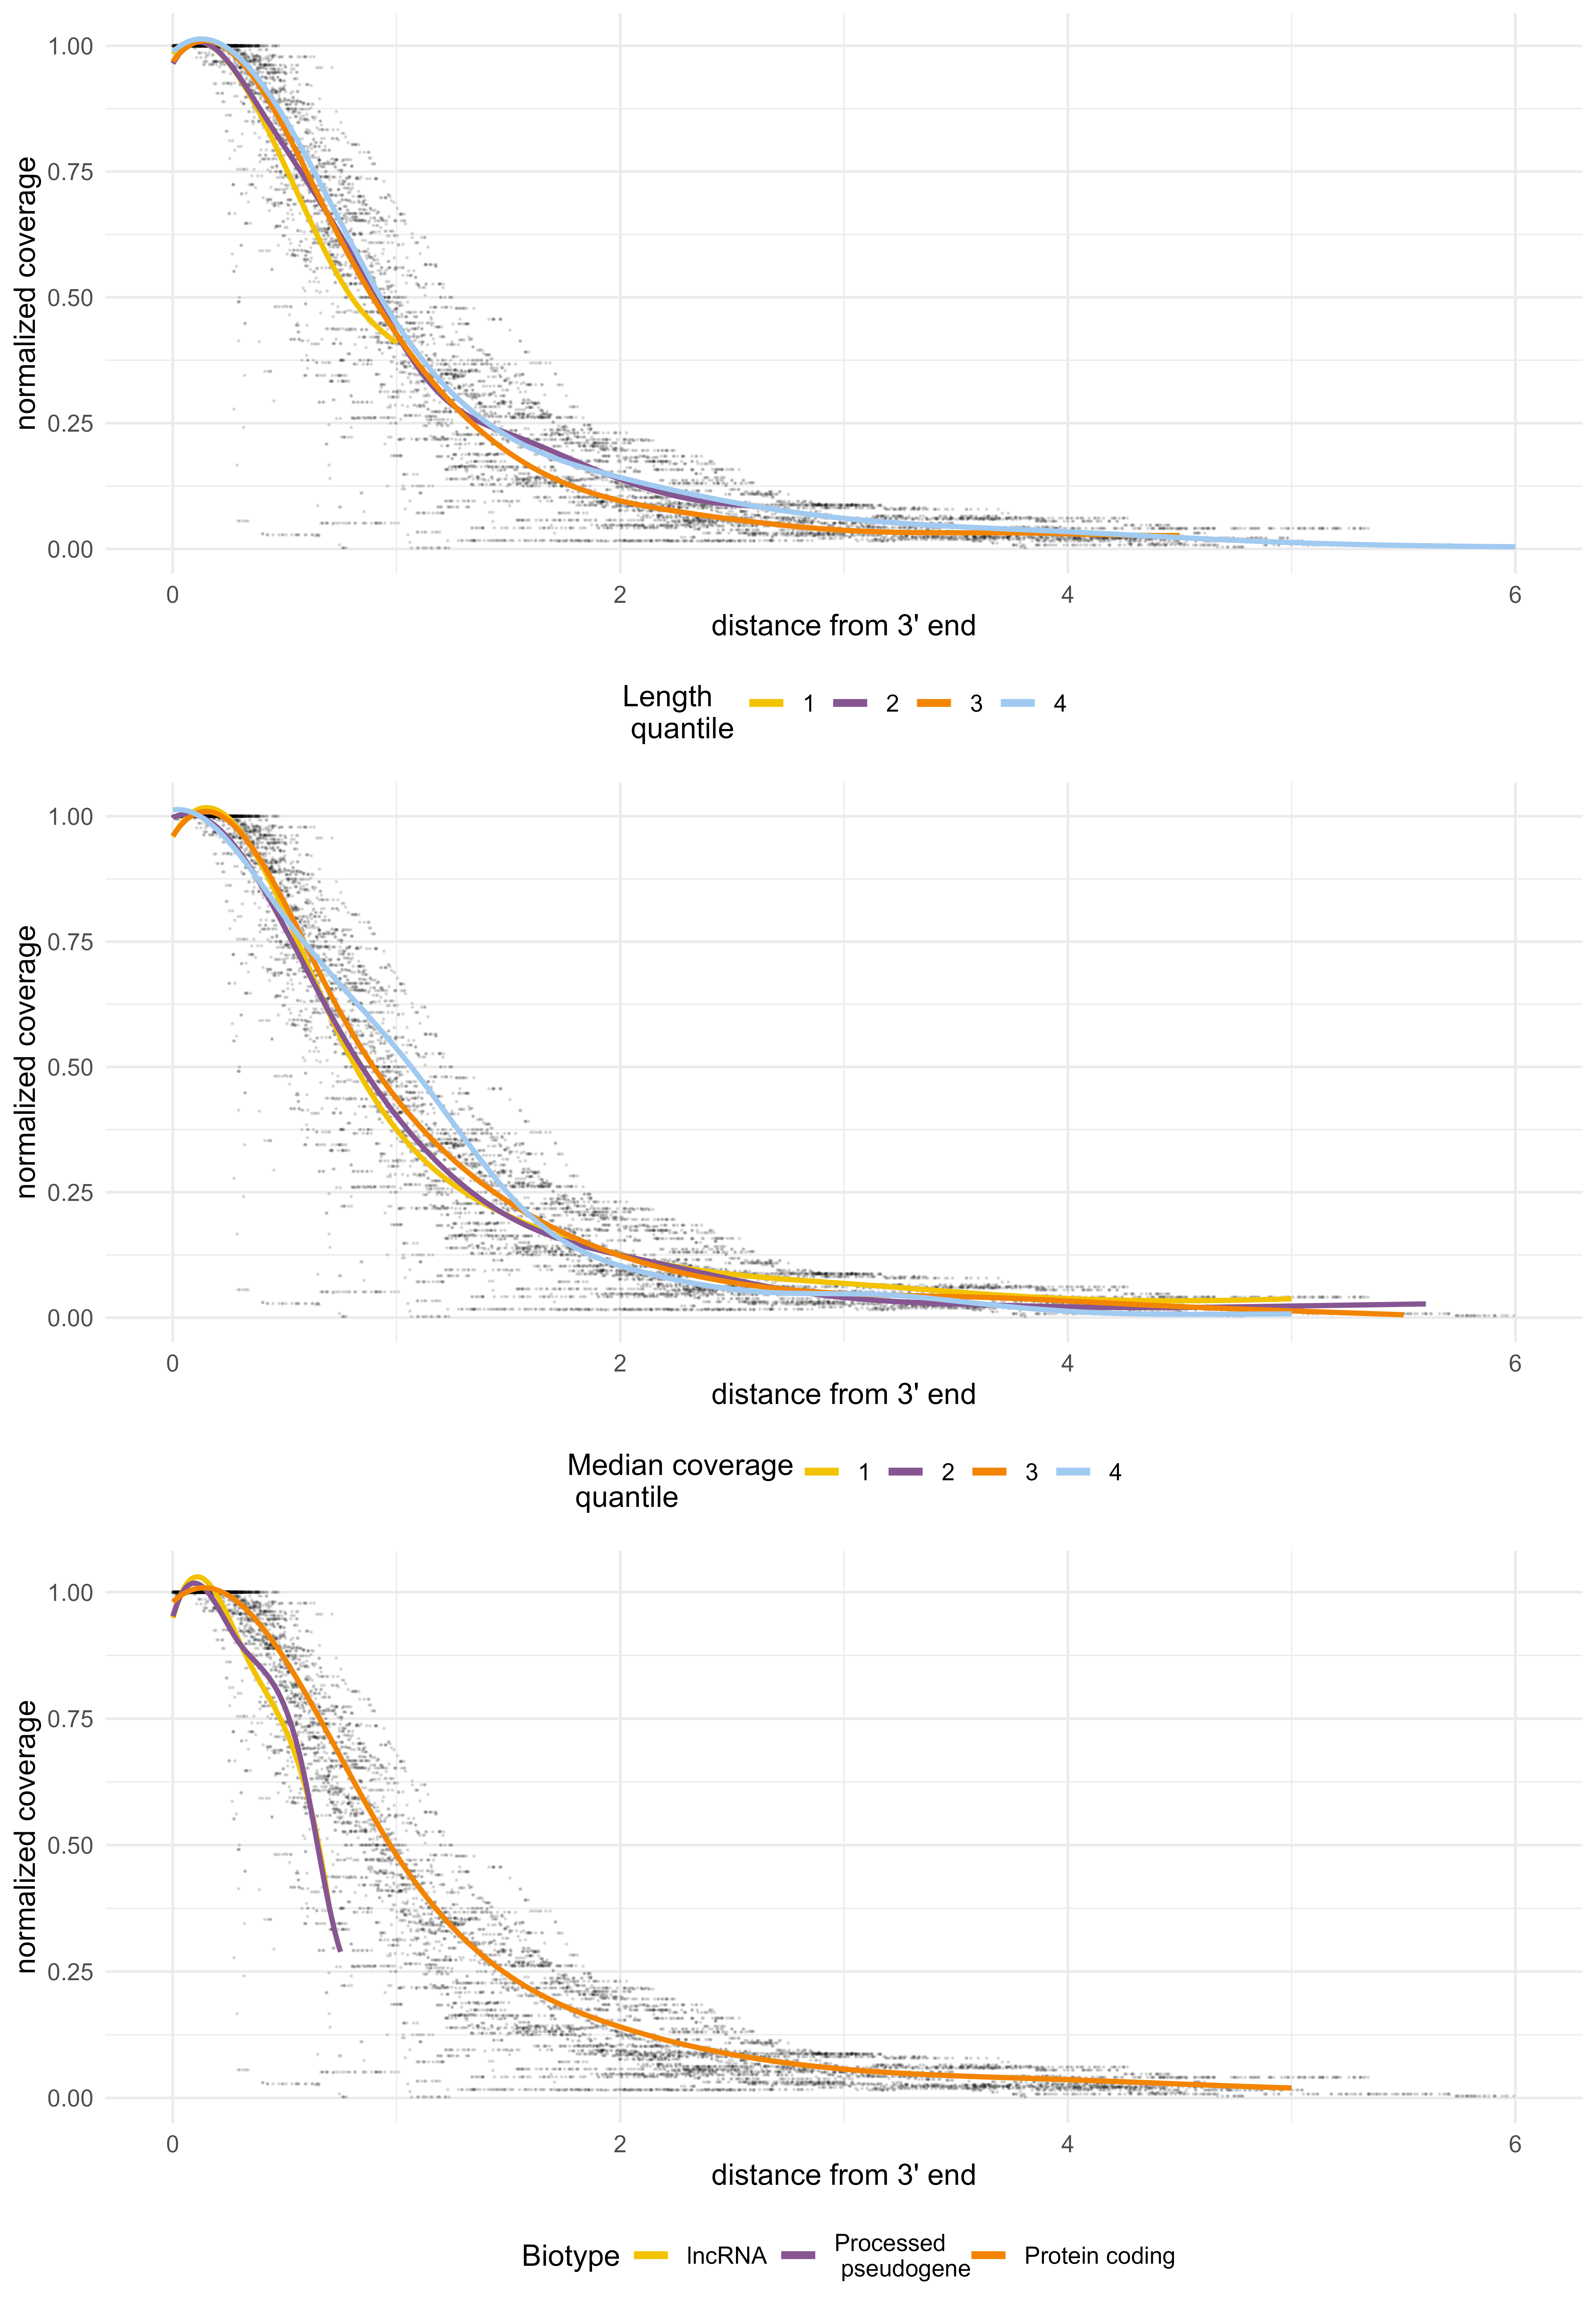
\includegraphics[width=\textwidth]{figures/sec-2-by-feature.png}
    \caption[Degradation curves in MCF7 striated by features]{Degradation curves in MCF7 striated by features. \textbf{a.} Degradation curves fit for isoforms within each length quantile separately, with quantiles 0\%:320,25\%:1360,50\%:2820,75\%:5590,100\%9038. \textbf{b.}   }
    \label{fig:cov-feature}
\end{figure}

\subsection{Degradation in spike-ins}

As discussed in the first chapter, the observed read truncation in ONT datasets may be a result of RNA degradation \textit{in vivo} or due to other extra-cellular factors including library preparation or sequencing artifacts. In this section, we analyse possible degradation in sequencing spike-ins, which are synthetic RNA molecules added to endogenous RNA samples before library preparation.   

\section{Read length-based degradation estimation}\label{sec:rld}

